%==============================================================================
%== template for LATEX poster =================================================
%==============================================================================
%
%--A0 beamer slide-------------------------------------------------------------
\documentclass[5pt, final]{beamer}
\usepackage[orientation=portrait, size=a0,
            scale=1.25         % font scale factor
           ]{beamerposter}
           
\geometry{
  hmargin=2.5cm, % little modification of margins
}

%
\usepackage[utf8]{inputenc}

\linespread{1.05}
%
%==The poster style============================================================
\usetheme{sharelatex}

%==Title, date and authors of the poster=======================================
\title
[Agile Vorgehensmodelle, Master, WS 202425] % Conference
{ % Poster title
	Die Rolle des Scrum Masters: Moderation, Konfliktlösung und Teamförderung
}

\author{ % Authors
	Nico Riedlinger\inst{1}, Marc Weiss\inst{1}
}
\institute
[Very Large University] % General University
{
	\inst{1} HTWG Konstanz
}
\date{\today}



\begin{document}
	\begin{frame}[t]
		%==============================================================================
		\begin{multicols}{3}
			%==============================================================================
			%==The poster content==========================================================
			%==============================================================================
			
			\section{Aufgabenbereich}
			
%			In Ref.~\cite{ref1}...
%			In Refs.~\cite{ref1,ref2}...
%			On webpage~\cite{web}...
			Der Aufgabenbereich eines Scrum Masters ist sehr vielseitig.
			Als Teil des Teams übernimmt er eine koordinierende Rolle und ist Ansprechpartner in Problemsituationen \cite{meindl12}.
			Diese können bezogen auf die technische Seite, zum Beispiel mit dem zu entwickelnden Produkt, oder auf sozialer Ebene sein.
			Bei Unstimmigkeiten im Team ist der Scrum Master dafür verantwortlich, diese Konflikte zu beseitigen. Insgesamt trägt er hauptsächlich zur Unterstützung des Teams, sowie zur Beseitigung von Hindernissen bei. \cite{Noll17}
			
			Eine Einordnung des Scrum Masters innerhalb des Teams ist in Figure \ref{fig:sm-team} zu sehen.
			Hier bildet er eine Schnittstelle vom Team nach außen gegenüber Managern.
			
			\vskip1ex
			\begin{figure}
				\centering
				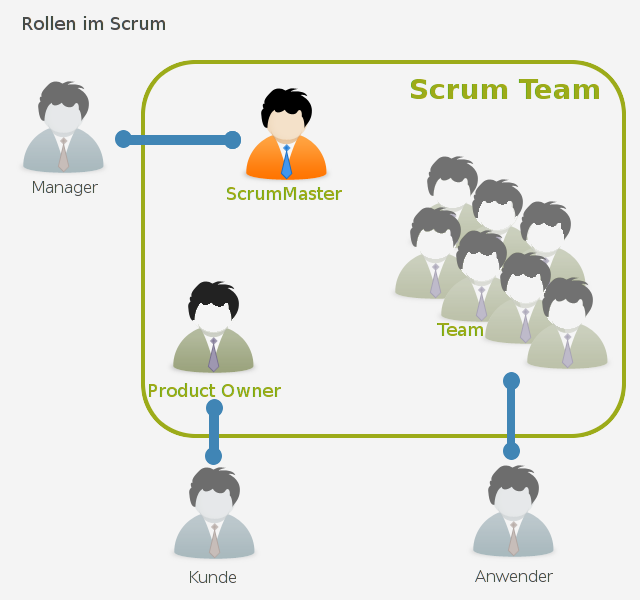
\includegraphics[width=0.95\columnwidth]{scrummaster}
				\caption{Einordnung des Scrum Masters innerhalb des gesamten Teams. Quelle: \cite{meindl12}}\label{fig:sm-team}
			\end{figure}
			\vskip2ex
		
			Des Weiteren ist er für die Organisation und Moderation von Besprechungen im Scrum-Kontext zuständig.
			Das umfasst sowohl das Sprint Planning als auch die Sprint Review sowie Retrospektive.
			Er verteilt im Voraus die jeweilige Agenda und moderiert die einzelnen Besprechungen.
			Letzteres gilt außerdem für das Daily Scrum.\cite{meindl12}
			
			\subsection{Moderation}
			
			Der Scrum Master moderiert die Besprechungen, um eine hohe Effektivität in der Teamkommunikation und das Erreichen der Ziele sicherzustellen \cite{vantighem24}.
			Unter korrektem Einsatz verschiedener Techniken kann die Qualität von Besprechungen wie auch die Motivation der Teilnehmer für eine solche Besprechung erheblich gesteigert werden.
			
			Eine der Techniken ist die Erstellung und Überprüfung von Teamregeln.
			Ähnlich wie die \textit{Definition of Done} oder \textit{Definition of Ready} für das Erstellen und Abschließen von User Storys, handelt es sich hierbei um einen dynamischen Regelsatz.
			Dieser kann je nach Aufgaben und Anforderungen des Teams in gemeinsamer Absprache angepasst werden.
			Der Scrum Master beobachtet das Team während Besprechungen und weist, ähnlich wie ein Schiedsrichter, auf Verstöße gegen die Regeln hin.
			Bei zu vielen Verstößen muss ein Grund dafür mit dem gesamten Team gefunden und gegebenenfalls das Regelwerk angepasst werden.
			
			% Moderation unabhängig von Führungsrolle durchführen, um Interessenskonflikte zu vermeiden.
            Weitere Techniken für eine gute Besprechungsqualität sind Timeboxing und neutrale Moderation \cite{malten24}.
            Beim Timeboxing geht es darum, die vorab kommunizierten Zeiten für eine Besprechung einzuhalten.
            Sowohl der Anfangszeitpunkt als auch das Ende sollten nicht überzogen werden.
            Wenn es dennoch mehr Gesprächsbedarf als verfügbare Zeit geben sollte, muss der Scrum Master als Moderator eine geeignete Lösung finden, ohne die Timebox zu überziehen.
            Als Beispiele dafür seien ein zusätzlicher Termin, persönliches Gespräch unter den Beteiligten oder eine Vertagung auf den nächsten regulären Besprechungstermin genannt.
            
            Diese Moderationsfähigkeiten sind besonders wichtig, um sicherzustellen, dass das Team die Scrum-Praktiken regelmäßig und effektiv umsetzt \cite{vantighem24}.
			
			\subsection{Konfliktlösung}
			
			Konflikte können das Teamklima und die Teamleistung negativ beeinflussen. Sie sind eine der schwierigsten Aufgaben für Scrum Master, wobei sie als neutrale Vermittler agieren \cite{Noll17}.
			Im Team können gemeinsame Erwartungen, Regeln und Strukturen festgelegt werden, um Konflikte vorzubeugen. Bei Auftretenden kleineren Spannungen versucht der Scrum Master diese frühzeitig zu erkennen und anzusprechen, damit sich daraus keine größeren Konflikte entwickeln. Bei eskalierten Konflikten interveniert der Scrum Master, wofür er verschiedene Rollen einnehmen kann. Als Moderator stellt er sicher, dass Gespräche strukturiert und vertraulich geführt werden. Als Berater unterstützt er unparteiisch bei einer Lösungsfindung. Als Leader kann er klare Vorgaben und Konsequenzen kommunizieren, wenn es nötig ist.
			Je nach Schwere des Konflikts kann das Vorgehen angepasst werden. Von der Vermittlung zwischen den Parteien, bis hin zur unterstützenden Einbindung disziplinarischer Führungskräfte oder Coaches. Neben der Deeskalation von Konflikten ist es wichtig eine aktive Konfliktkultur zu fördern, damit Meinungsverschiedenheiten offen ausgetragen werden können, woran das Team wächst. \cite{Anker23}
			
			\subsection{Teamförderung}
			
			Die Förderung des Teams ist ein zentraler Bestandteil der Rolle des Scrum Masters.
            Dies beinhaltet die Unterstützung des Teams bei der Selbstorganisation und Übernahme von Führungsrollen, während das Team reift. Scrum Master tragen zur Dynamik und zum Wohlbefinden des Teams bei, indem sie das Team herausfordern, seine Leistung zu steigern und zu einem guten internen Teamklima unterstützend beitragen \cite{Spiegler21}.
            
            Als Technik zur Teamförderung können agile Spiele eingesetzt werden.
            Bleß und Wagner \cite{bless24} führen viele verschiedene auf.
            Sie lassen sich in mehrere Kategorien unterteilen, so zum Beispiel Teambuilding/Teamwork, Selbstorganisation oder Multitasking.
            Solche Spiele können sowohl in neu zusammengefundenen Teams zum Kennenlernen als auch in bereits länger bestehenden Teams zur Festigung oder Verbesserung des Scrum-Prozesses eingesetzt werden.
            Üblicherweise nutzen sie das Teambuilding oder eine Komponente von Scrum auf einer höheren Abstraktionsebene aus und verwenden viele Metaphern.
            Ein Spiel, was besonders das iterative und inkrementelle Vorgehen von Scrum vermittelt, ist die \textit{Marshmallow Challenge}.
            Es geht darum, einen höchstmöglichen Turm aus rohen Spaghetti zu bauen und auf der Spitze ein Marshmallow zu platzieren.
            Die Entwürfe der Teams werden in der Regel mehrfach überarbeitet und ausgebaut bis das finale Produkt steht.\cite{bless24}
			
			\section {Führungsverhalten}
            
            Ein Scrum Master ist für das Team eine dienende Führungskraft, aber kein Projektleiter. Er gibt dem Team weder Arbeitsanweisungen, noch beurteilt er Teammitglieder. In der Literatur wird die Führungsrolle oft als Empowering Leadership, Servant Leadership oder als Coach bezeichnet \cite{Spiegler21}\cite{Frye24}. Der Scrum Master achtet dabei speziell bei der Formung von Scrum Teams auf die Einhaltung der Scrum Prinzipien und ermöglicht dem Team durch Unterstützung und Beseitigung von Hindernissen effektives Arbeiten. 
            Wichtige Führungskompetenzen des Scrum Masters sind organisatorische und kommunikative Kompetenzen, sowie die Fähigkeit Konflikte zu managen. Dies erfordert Vertrauen und gute Beziehungen zu den Teammitgliedern. Darüber hinaus achtet er auf das Wissensmanagement und die Selbstorganisation im Team.\cite{Frye24} 
            Entscheidungen werden im Sinne der Selbstorganisation dem Team überlassen, das sich theoretisch vollständig selbst führen soll. Das Führungsverhalten des Scrum Masters ändert sich situativ, während das Team reift. \cite{Spiegler21}
			
			\section{Abgrenzung zum Product Owner}
			
			% Scrum Master vs. Product Owner
            Die Rollen des Scrum Masters und Product Owners werden oftmals miteinander vermischt, teilweise sogar von der gleichen Person ausgeführt, was aufgrund der unterschiedlichen Aufgabenbereiche zu Interessenskonflikten führen kann. % eine Person, zwei Rollen = Interessenskonflikte
            Beide Rollen haben sehr unterschiedliche Verantwortlichkeiten und Charakteristiken \cite{sutherland14}.
            
            % kurzer Abriss von PO
            Diese Unterschiede sind bereits in Figure \ref{fig:sm-team} zu sehen.
            Während sich der Scrum Master um das Team kümmert und versucht, mögliche Blockaden zu beseitigen, ist der Product Owner am entstehenden Produkt interessiert und aus Sicht des Kunden verantwortlich \cite{Spiegler21}.         
            Der Scrum Master hingegen bildet eine Art \textit{Vertrauensperson} bei Problemen gegenüber dem Team.
            Würde die Vertraunsperson gleichzeitig für den Erfolg des Produkts verantwortlich sein, müsste sie sich in Konfliktsituationen entscheiden, ob sie sich mehr für das Team, oder mehr für das Produkt einsetzt.
            Dadurch würde ein Misstrauen gegenüber des Scrum Masters bzw. Product Owners entstehen \cite{me-company}. Infolgedessen werden Probleme nie behoben und im schlimmsten Fall zerfällt das Team.
			
			% Er steht in konstantem Austausch zu den Kunden, nimmt deren Anforderungen auf und diskutiert diese.
			%            Anschließend zerkleinert der Product Owner die Anforderungen in einzelne Teile und formuliert sie als User Story.
			%            Auf Basis dieser User Storys kann er nun dem Entwicklungsteam das weitere Vorgehen präsentieren.
			
			%            Da der Scrum Master eigentlich für die Probleme des Teams und die Beseitigung derer zuständig ist, fungiert er auch als eine Art \textit{Vertrauensperson} in Problemfällen.
			
			%            Die Teammitglieder können sich nicht mehr mit ihren Problemen an die Vertrauensperson wenden.
			
			\section{Ergebnisse}
			Zusammengefasst sind folgende die zentralen Verantwortlichkeiten des Scrum Masters:
            \begin{itemize}
    			\item Steigerung der Produktivität des Teams \cite{vantighem24}.
    			\item Moderieren, Team fördern und Konflikte beseitigen.
    			\item Abschirmung nach außen, wie zum Management \cite{meindl12}.
                \item Einhaltung der Scrum Prinzipien, da nicht automatisch 'twice as much in half as much time' nur durch Scrum Einführung ermöglicht wird \cite{sutherland14}.
                \item Klare Rollentrennung zwischen Scrum Master und Product Owner.
            \end{itemize}
			
%			\vskip1ex
%			\begin{table}
%				\centering
%				\caption{This is a table with scientific results.}
%				\begin{tabular}{ccccc}
%					\hline\hline
%					1 & 2 & 3 & 4 & 5\\
%					\hline
%					aaa & bbb & ccc & ddd & eee\\
%					aaaa & bbbb & cccc & dddd & eeee\\
%					aaaaa & bbbbb & ccccc & ddddd & eeeee\\
%					aaaaaa & bbbbbb & cccccc & dddddd & eeeeee\\
%					1.000 & 2.000 & 3.000 & 4.000 & 5.000\\
%					\hline\hline
%				\end{tabular}
%			\end{table}
%			\vskip2ex
			
			%==============================================================================
			%==End of content==============================================================
			%==============================================================================
			
			%--References------------------------------------------------------------------
			
			\subsection{References}
						
			\begin{thebibliography}{99}
				
%				\bibitem{ref1} J.~Doe, Article name, \textit{Phys. Rev. Lett.}
%				
%				\bibitem{ref2} J.~Doe, J.~Smith, Other article name, \textit{Phys. Rev. Lett.}
%				
%				\bibitem{web} \url{http://www.google.pl}
				
				\bibitem{Anker23} P. Anker (2023), Konflikte Meistern: Handbuch für Scrum Master in Agilen Teams. \textit{tredition}
				
				\bibitem{bless24} M.~Bleß, D.~Wagner (2024), Agile Spiele - kurz \& gut . 2. Auflage. \textit{O'Reilly Verlag GmbH \& Co. KG}.
				
				\bibitem{Frye24} M.~Frye, H.~Möltner (2024), Selbstorganisiert und dennoch geführt – eine explorative Studie zur Führung durch Scrum Master. In: GIO, Zeitschrift für Angewandte Organisationspsychologie, 55, S. 607–617 \textit{Springer}
				
				\bibitem{malten24} M.~Malten (2024), Effektive Team-Meetings: Impulse aus der agilen Praxis für bessere Besprechungen und Kommunikation. 1. Auflage. \textit{Springer Gabler Berlin, Heidelberg}.
				
				\bibitem{meindl12} C.~Meindl, Der ScrumMaster, \url{https://alphanodes.com/de/der-scrummaster} (zul. besucht am 10.12.2024)
				
				\bibitem{me-company} Me~\&~Company~GmbH, Scrum Master: Coach, Moderator und Unterstützer, \url{https://www.me-company.de/magazin/scrum-master/} (zul. besucht am 10.12.2024)
				
				\bibitem{Noll17} J.~Noll, M.~Razzak, J~Bass, S.~Beecham (2017), A Study of the Scrum Master's Role. In. Product-Focused Software Process Improvement. S.307-323 \textit{Springer, Cham}
								
				\bibitem{Spiegler21} S.~Spiegler, C.~Heinecke, S.~Wagner (2021), An empirical study on changing leadership in agile teams. 
				\textit{Empirical Software Engineering. 26. Auflage.}
						                
                \bibitem{sutherland14} J.~Sutherland, JJ~Sutherland (2014), Scrum: The Art of Doing Twice the Work in Half the Time. \textit{Crown Currency}.
                
                \bibitem{vantighem24} C.~Vantighem, Der Scrum Master: Definition, Aufgaben und Nutzen, \url{https://www.teammeter.com/de/scrum-master-aufgaben-verantwortung-und-nutzen} (zul. besucht am 10.12.2024)            
 
                
               
				
			\end{thebibliography}
			%--End of references-----------------------------------------------------------
			
		\end{multicols}
		
		%==============================================================================
	\end{frame}
\end{document}
